\documentclass{standalone}
\usepackage{tikz}
\usetikzlibrary{arrows, decorations.markings}

% for double arrows a la chef
% adapt line thickness and line width, if needed
\tikzstyle{vecArrow} = [thick, decoration={markings,mark=at position
   1 with {\arrow[line width=0.1pt, fill=green, scale=3]{triangle 60}}},
   double distance=5.6pt, shorten >= 5.6pt,
   preaction = {decorate},
   postaction = {draw,line width=5.6pt, gray, shorten >= 5.6pt}
   ]
\tikzstyle{innerWhite} = [semithick, black!50, line width=5.6pt, shorten >= 5.5pt]

\begin{document}

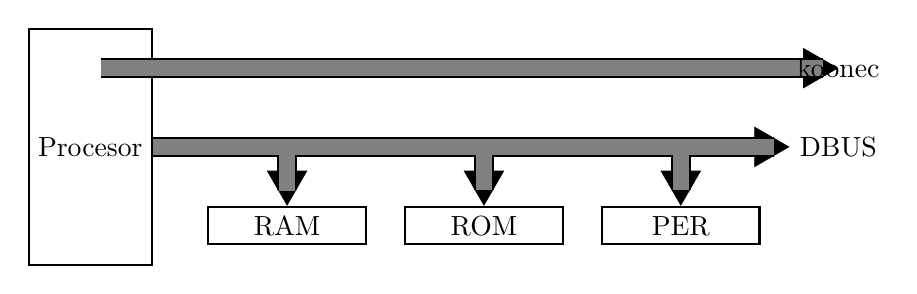
\begin{tikzpicture}[thick]
  \node[draw,rectangle, minimum height=3cm] (node_CPU) {Procesor};
  \node[inner sep=0,minimum size=0,right of=node_CPU, xshift=1.5cm] (k) {}; % invisible node
  \node[inner sep=0,minimum size=0,right of=k, xshift=1.5cm] (l) {}; % invisible node
  \node[inner sep=0,minimum size=0,right of=l, xshift=1.5cm] (m) {}; % invisible node

  \node[draw,rectangle, minimum width=2cm, below of=k] (c) {RAM};
  \node[draw,rectangle, minimum width=2cm, below of=l] (d) {ROM};
  \node[draw,rectangle, minimum width=2cm, below of=m] (e) {PER};
  \node[right of=m, xshift=1cm] (end_DBUS) {DBUS};
  
  % 1st pass - DBUS: draw arrows
  \draw[vecArrow] (node_CPU) to (end_DBUS);
  \draw[vecArrow] (k) -- (c);
  \draw[vecArrow] (l) -- (d);
  \draw[vecArrow] (m) -- (e);

  % 2nd pass: copy all from 1st pass, and replace vecArrow with innerWhite
  \draw[innerWhite] (node_CPU) to (end_DBUS);
  \draw[innerWhite] (k) to (c);

  % Note: If you have no branches, the 2nd pass is not needed
  \node[above of=node_CPU] (kk) {};
  \draw[vecArrow] (kk) to ([yshift=1cm]end_DBUS);
    
    \node[right of=m, xshift=1cm, yshift=1cm] (end_DBUS) {koonec};

\end{tikzpicture}

\end{document}